\documentclass{clseminar}

    \usepackage{tikz}
    \usepackage{soul}

    % \documentclass{clseminar}

    \usepackage{tikz}
    \usepackage{soul}

    % \documentclass{clseminar}

    \usepackage{tikz}
    \usepackage{soul}

    % \documentclass{clseminar}

    \usepackage{tikz}
    \usepackage{soul}

    % \input{../PREAMBLE/Drawings}

\begin{document}

\begin{figure}
    \begin{center}
\input{../DRAWINGS/ProperOrder}
\caption{Proper orders on terms}
    \end{center}
\end{figure}

\begin{figure}
    \begin{center}
\input{../DRAWINGS/PartialOrder}
\caption{Equivalence relation vs.~partial order}
\end{center}
\end{figure}

\end{document}

\begin{document}

\begin{figure}
    \begin{center}
\begin{tikzpicture}
    \node (defCUC) at (-4,8.5) { \( s\succ t\Rightarrow \ctx[s]\succ \ctx[t] \)};
    \node (CUC) at (-4,8) { contexts };
    \node (defCUS) at (0,8.5) { \( s\succ t\Rightarrow s\sigma\succ t\sigma \)};
    \node (CUS) at (0,8) { substitutions };

    \node (ASYM) at (4,8.5) { \( s\succ t\Rightarrow t\not\succ s \) };
    \node (ASYM) at (4,8) { asymmetric };

        \node (CL) at (-2,6) { closed under };
        \node (defIRR) at (2,6.5) { \( s\succ t\succ u\Rightarrow s\succ u \) };
        \node (IRR) at (6,6) { irreflexive };
        \node (defIRR) at (6,6.5) { \( s\nsucc s \) };
        \node (TRA) at (2,6) { transitive };

        \node (POx) at (4,4.4) { \( > \) };
        \node (PO) at (4,4) { proper order };
        \node (RWRx) at (0,4.4) { \( \rightarrow^*_\mcR \) };
        \node (RWR) at (0,4) { rewrite relation };

        \node (defSTP) at (-2,2.5) { \( \ctx\neq\ctxhole\Rightarrow \ctx[s]\succ s \) };
        \node (STP) at (-2,2) { subterm property };
        \node (RWO) at (2,2) { rewrite order };
        \node (defWF) at (8,4.5) { \( \nexists s_0(s_i\succ s_{i+1})_{i=0}^{\infty} \) };
        \node (WF) at (8,4) { well-founded };

        \node (SO) at (0,0) {simplification order};
        \node (RO) at (4,0) {reduction order};

        \node (WFO) at (6,2) { well-founded order };


        \draw[->] (CL) -- (CUC);
        \draw[->] (CL) -- (CUS);

        \draw[->] (PO) -- (IRR);
        \draw[->] (PO) -- (TRA);

        \draw[->] (RWR) -- (CL);

        \draw[->] (RWO) -- (PO);
        \draw[->] (RWO) -- (RWR);

        \draw[->] (SO) -- (STP);
        \draw[->] (RO) -- (RWO);
        \draw[->] (RO) -- (WFO);
        % \draw (RO) edge[out=0,in=-45,->] (WF);

        \draw[->] (SO) -- (RWO);
        \draw[->, dotted] (SO) -- (RO);

        \draw[->] (WFO) -- (WF);
        \draw[->] (WFO) -- (PO);

        \draw[->, dotted] (WF) -- (IRR);

        % \node (TRAIRR) at (4,7) { \( \bullet \) };
        \draw[->, dotted] (4,7) -- (ASYM);

        \draw[dotted] (TRA) edge [out=-10, in=-90] (4,7);
        \draw[dotted] (IRR) edge [out=190, in=-90] (4,7);

        \draw[->, dotted] (ASYM) -- (IRR);
        % \draw[->, dotted] (ASYM) edge [out=0, in=0] (IRR);


    \end{tikzpicture}
\caption{Proper orders on terms}
    \end{center}
\end{figure}

\begin{figure}
    \begin{center}
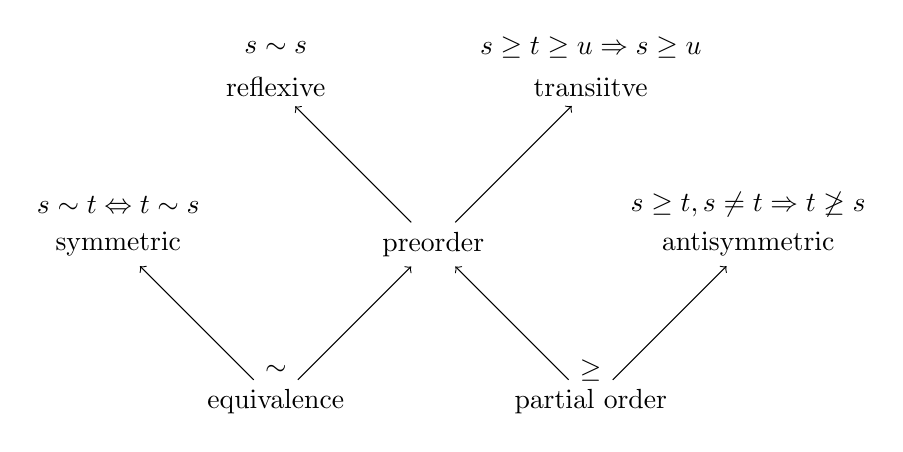
\begin{tikzpicture}
    \node (defREFLEXIVE) at (-2,2.5) { $s\sim s$ };
    \node (REFLEXIVE) at (-2,2) { reflexive };

    \node (defTRANSITIVE) at (2,2.5) { $s\geq t\geq u\Rightarrow s\geq u$ };
    \node (TRANSITIVE) at (2,2) { transiitve };

    \node (defTRANSITIVE) at (-4,0.5) { $s\sim t\Leftrightarrow t\sim s$ };
    \node (SYMMETRIC) at (-4,0) { symmetric };
    \node (PREORDER) at (0,0) { preorder };

    \node (defANTISYMMETRIC) at (4,0.5) { $s\geq t, s\neq t \Rightarrow t\not\geq s$ };
    \node (ANTISYMMETRIC) at (4,0) { antisymmetric };
    \node (SIM) at (-2,-1.6) { $\sim$ };
    \node (EQUIVALENCE) at (-2,-2) { equivalence };
    \node (GEQ) at (2,-1.6) { $\geq$ };
    \node (PARTIAL) at (2,-2) { partial order };

    \draw[->] (PREORDER) -- (REFLEXIVE);
    \draw[->] (PREORDER) -- (TRANSITIVE);

    \draw[->] (EQUIVALENCE) -- (SYMMETRIC);
    \draw[->] (EQUIVALENCE) -- (PREORDER);
    \draw[->] (PARTIAL) -- (PREORDER);
    \draw[->] (PARTIAL) -- (ANTISYMMETRIC);
\end{tikzpicture}
\caption{Equivalence relation vs.~partial order}
\end{center}
\end{figure}

\end{document}

\begin{document}

\begin{figure}
    \begin{center}
\begin{tikzpicture}
    \node (defCUC) at (-4,8.5) { \( s\succ t\Rightarrow \ctx[s]\succ \ctx[t] \)};
    \node (CUC) at (-4,8) { contexts };
    \node (defCUS) at (0,8.5) { \( s\succ t\Rightarrow s\sigma\succ t\sigma \)};
    \node (CUS) at (0,8) { substitutions };

    \node (ASYM) at (4,8.5) { \( s\succ t\Rightarrow t\not\succ s \) };
    \node (ASYM) at (4,8) { asymmetric };

        \node (CL) at (-2,6) { closed under };
        \node (defIRR) at (2,6.5) { \( s\succ t\succ u\Rightarrow s\succ u \) };
        \node (IRR) at (6,6) { irreflexive };
        \node (defIRR) at (6,6.5) { \( s\nsucc s \) };
        \node (TRA) at (2,6) { transitive };

        \node (POx) at (4,4.4) { \( > \) };
        \node (PO) at (4,4) { proper order };
        \node (RWRx) at (0,4.4) { \( \rightarrow^*_\mcR \) };
        \node (RWR) at (0,4) { rewrite relation };

        \node (defSTP) at (-2,2.5) { \( \ctx\neq\ctxhole\Rightarrow \ctx[s]\succ s \) };
        \node (STP) at (-2,2) { subterm property };
        \node (RWO) at (2,2) { rewrite order };
        \node (defWF) at (8,4.5) { \( \nexists s_0(s_i\succ s_{i+1})_{i=0}^{\infty} \) };
        \node (WF) at (8,4) { well-founded };

        \node (SO) at (0,0) {simplification order};
        \node (RO) at (4,0) {reduction order};

        \node (WFO) at (6,2) { well-founded order };


        \draw[->] (CL) -- (CUC);
        \draw[->] (CL) -- (CUS);

        \draw[->] (PO) -- (IRR);
        \draw[->] (PO) -- (TRA);

        \draw[->] (RWR) -- (CL);

        \draw[->] (RWO) -- (PO);
        \draw[->] (RWO) -- (RWR);

        \draw[->] (SO) -- (STP);
        \draw[->] (RO) -- (RWO);
        \draw[->] (RO) -- (WFO);
        % \draw (RO) edge[out=0,in=-45,->] (WF);

        \draw[->] (SO) -- (RWO);
        \draw[->, dotted] (SO) -- (RO);

        \draw[->] (WFO) -- (WF);
        \draw[->] (WFO) -- (PO);

        \draw[->, dotted] (WF) -- (IRR);

        % \node (TRAIRR) at (4,7) { \( \bullet \) };
        \draw[->, dotted] (4,7) -- (ASYM);

        \draw[dotted] (TRA) edge [out=-10, in=-90] (4,7);
        \draw[dotted] (IRR) edge [out=190, in=-90] (4,7);

        \draw[->, dotted] (ASYM) -- (IRR);
        % \draw[->, dotted] (ASYM) edge [out=0, in=0] (IRR);


    \end{tikzpicture}
\caption{Proper orders on terms}
    \end{center}
\end{figure}

\begin{figure}
    \begin{center}
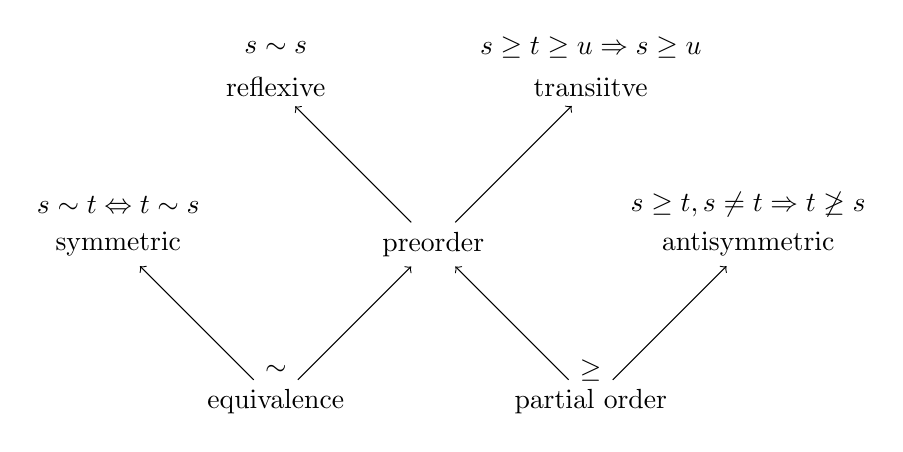
\begin{tikzpicture}
    \node (defREFLEXIVE) at (-2,2.5) { $s\sim s$ };
    \node (REFLEXIVE) at (-2,2) { reflexive };

    \node (defTRANSITIVE) at (2,2.5) { $s\geq t\geq u\Rightarrow s\geq u$ };
    \node (TRANSITIVE) at (2,2) { transiitve };

    \node (defTRANSITIVE) at (-4,0.5) { $s\sim t\Leftrightarrow t\sim s$ };
    \node (SYMMETRIC) at (-4,0) { symmetric };
    \node (PREORDER) at (0,0) { preorder };

    \node (defANTISYMMETRIC) at (4,0.5) { $s\geq t, s\neq t \Rightarrow t\not\geq s$ };
    \node (ANTISYMMETRIC) at (4,0) { antisymmetric };
    \node (SIM) at (-2,-1.6) { $\sim$ };
    \node (EQUIVALENCE) at (-2,-2) { equivalence };
    \node (GEQ) at (2,-1.6) { $\geq$ };
    \node (PARTIAL) at (2,-2) { partial order };

    \draw[->] (PREORDER) -- (REFLEXIVE);
    \draw[->] (PREORDER) -- (TRANSITIVE);

    \draw[->] (EQUIVALENCE) -- (SYMMETRIC);
    \draw[->] (EQUIVALENCE) -- (PREORDER);
    \draw[->] (PARTIAL) -- (PREORDER);
    \draw[->] (PARTIAL) -- (ANTISYMMETRIC);
\end{tikzpicture}
\caption{Equivalence relation vs.~partial order}
\end{center}
\end{figure}

\end{document}

\begin{document}



\providecommand{\ctx}{C}
\providecommand{\ctxhole}{[]}

\begin{figure}
    \begin{center}
\begin{tikzpicture}
    \node (defCUC) at (-4,8.5) { \( s\succ t\Rightarrow \ctx[s]\succ \ctx[t] \)};
    \node (CUC) at (-4,8) { contexts };
    \node (defCUS) at (0,8.5) { \( s\succ t\Rightarrow s\sigma\succ t\sigma \)};
    \node (CUS) at (0,8) { substitutions };

    \node (ASYM) at (4,8.5) { \( s\succ t\Rightarrow t\not\succ s \) };
    \node (ASYM) at (4,8) { asymmetric };

        \node (CL) at (-2,6) { closed under };
        \node (defIRR) at (2,6.5) { \( s\succ t\succ u\Rightarrow s\succ u \) };
        \node (IRR) at (6,6) { irreflexive };
        \node (defIRR) at (6,6.5) { \( s\nsucc s \) };
        \node (TRA) at (2,6) { transitive };

        \node (POx) at (4,4.4) { \( > \) };
        \node (PO) at (4,4) { proper order };
        \node (RWRx) at (0,4.4) { \( \rightarrow^*_\mcR \) };
        \node (RWR) at (0,4) { rewrite relation };

        \node (defSTP) at (-2,2.5) { \( \ctx\neq\ctxhole\Rightarrow \ctx[s]\succ s \) };
        \node (STP) at (-2,2) { subterm property };
        \node (RWO) at (2,2) { rewrite order };
        \node (defWF) at (8,4.5) { \( \nexists s_0(s_i\succ s_{i+1})_{i=0}^{\infty} \) };
        \node (WF) at (8,4) { well-founded };

        \node (SO) at (0,0) {simplification order};
        \node (RO) at (4,0) {reduction order};

        \node (WFO) at (6,2) { well-founded order };


        \draw[->] (CL) -- (CUC);
        \draw[->] (CL) -- (CUS);

        \draw[->] (PO) -- (IRR);
        \draw[->] (PO) -- (TRA);

        \draw[->] (RWR) -- (CL);

        \draw[->] (RWO) -- (PO);
        \draw[->] (RWO) -- (RWR);

        \draw[->] (SO) -- (STP);
        \draw[->] (RO) -- (RWO);
        \draw[->] (RO) -- (WFO);
        % \draw (RO) edge[out=0,in=-45,->] (WF);

        \draw[->] (SO) -- (RWO);
        \draw[->, dotted] (SO) -- (RO);

        \draw[->] (WFO) -- (WF);
        \draw[->] (WFO) -- (PO);

        \draw[->, dotted] (WF) -- (IRR);

        % \node (TRAIRR) at (4,7) { \( \bullet \) };
        \draw[->, dotted] (4,7) -- (ASYM);

        \draw[dotted] (TRA) edge [out=-10, in=-90] (4,7);
        \draw[dotted] (IRR) edge [out=190, in=-90] (4,7);

        \draw[->, dotted] (ASYM) -- (IRR);
        % \draw[->, dotted] (ASYM) edge [out=0, in=0] (IRR);


    \end{tikzpicture}
\caption{Proper orders on terms}
    \end{center}
\end{figure}

\begin{figure}
    \begin{center}
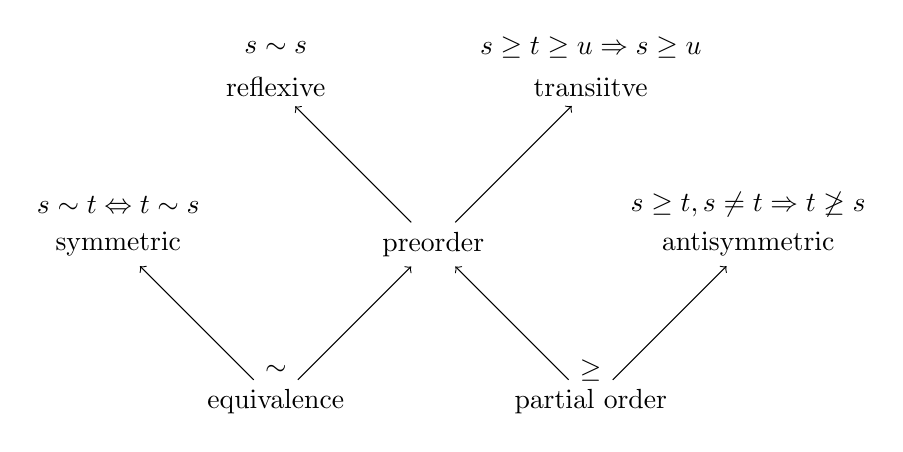
\begin{tikzpicture}
    \node (defREFLEXIVE) at (-2,2.5) { $s\sim s$ };
    \node (REFLEXIVE) at (-2,2) { reflexive };

    \node (defTRANSITIVE) at (2,2.5) { $s\geq t\geq u\Rightarrow s\geq u$ };
    \node (TRANSITIVE) at (2,2) { transiitve };

    \node (defTRANSITIVE) at (-4,0.5) { $s\sim t\Leftrightarrow t\sim s$ };
    \node (SYMMETRIC) at (-4,0) { symmetric };
    \node (PREORDER) at (0,0) { preorder };

    \node (defANTISYMMETRIC) at (4,0.5) { $s\geq t, s\neq t \Rightarrow t\not\geq s$ };
    \node (ANTISYMMETRIC) at (4,0) { antisymmetric };
    \node (SIM) at (-2,-1.6) { $\sim$ };
    \node (EQUIVALENCE) at (-2,-2) { equivalence };
    \node (GEQ) at (2,-1.6) { $\geq$ };
    \node (PARTIAL) at (2,-2) { partial order };

    \draw[->] (PREORDER) -- (REFLEXIVE);
    \draw[->] (PREORDER) -- (TRANSITIVE);

    \draw[->] (EQUIVALENCE) -- (SYMMETRIC);
    \draw[->] (EQUIVALENCE) -- (PREORDER);
    \draw[->] (PARTIAL) -- (PREORDER);
    \draw[->] (PARTIAL) -- (ANTISYMMETRIC);
\end{tikzpicture}
\caption{Equivalence relation vs.~partial order}
\end{center}
\end{figure}

\end{document}